\chapter{FFT}
\label{FFT}
\section{Notizen}

vorbereitung:\\
Eulers identity, complex numbers.



Initialisierung
Fourier transformation.
Spectral filter
Spectral Reverb, delay.
Windowing
Convolution,
evtl. cross correlation
freq. crossover
spectral synyth,
spectraum display.


evtl auch:
\begin{itemize}
	\item send / receive, send / receive bei gui objekten.
	\item initialisierung
	\item 
\end{itemize}


Diskretes Signal -> Periodisches Spectrum \\
Periodisches Signal -> Diskretes Spectrum

gute referenz:
http://jackschaedler.github.io/circles-sines-signals


\begin{figure}[h]
	\begin{center}
		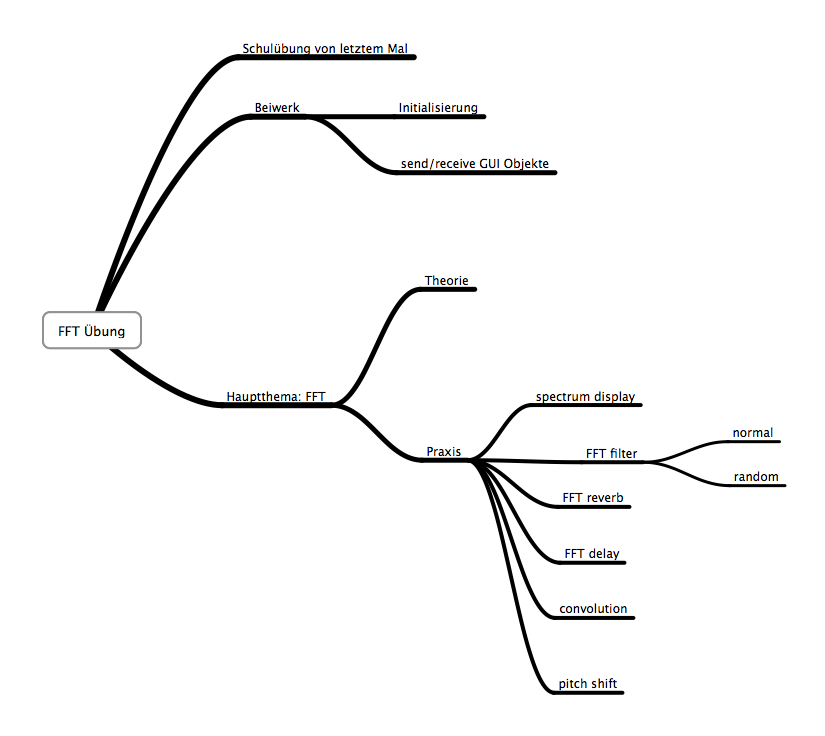
\includegraphics[width = 14cm]{img/FFToverview.png}
		\caption{caption}
		\label{fig:name}
	\end{center}
\end{figure}

\section{Fourier Transformation}

Geschichte:
Bernoulli, Euler, Gauß, Fourier

Eulers identität:
\begin{equation}
	e ^{ix} = cos(x)+i \cdot sin(x)
\end{equation}

Fourier Transformation:\\
\begin{equation}
	X(f)= \mathcal{F} \{x(t)\} = \int_{-\infty}^\infty \! x(t) e^{-j2\pi ft} \, \mathrm{d}t
\end{equation}

Inverse Fourier Transformation:\\
\begin{equation}
	x(t)= \mathcal{F}^{-1} \{X(f)\} = \int_{-\infty}^\infty \! X(f) e^{j2\pi ft} \, \mathrm{d}f
\end{equation}

\begin{figure}[h]
	\begin{center}
		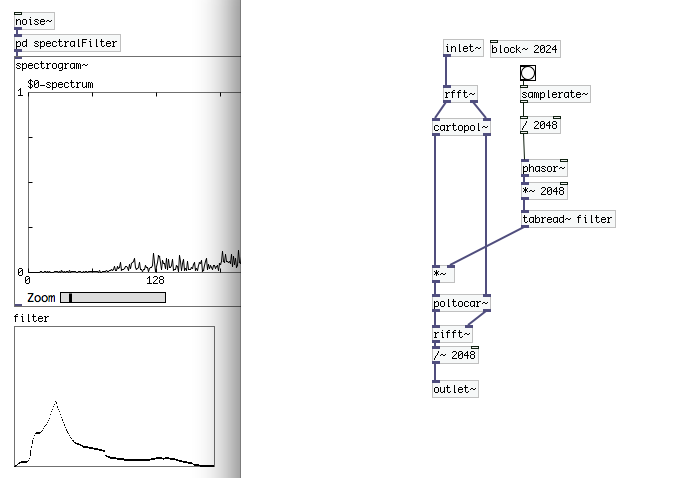
\includegraphics[width = 14cm]{img/spectralFilter.png}
		\caption{spectralFilter.pd}
		\label{fig:spectralFilter}
	\end{center}
\end{figure}

\begin{figure}[h]
	\begin{center}
		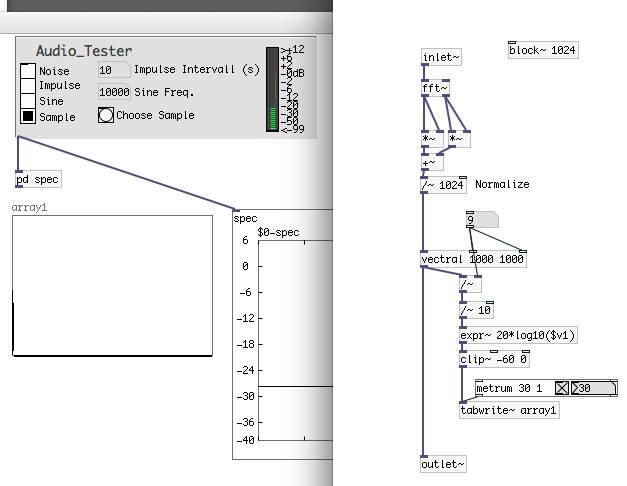
\includegraphics[width = 14cm]{img/showspectrum.png}
		\caption{showspectrum}
		\label{fig:showspectrum}
	\end{center}
\end{figure}
